\setlength{\parindent}{0pt}

\section*{Задание 1}
\textf{Исследовать данную функцию на равномерную непрерывность на данном мно жестве пользуясь определением.\\}
{\large
    \[
        f(x) = 2x - \sqrt{x} + \frac{1}{x - 1},\ a)X = [2, +\infty), \ b)X = (0, 1)
    \]
}
\textbf{\Large Решение:\\}

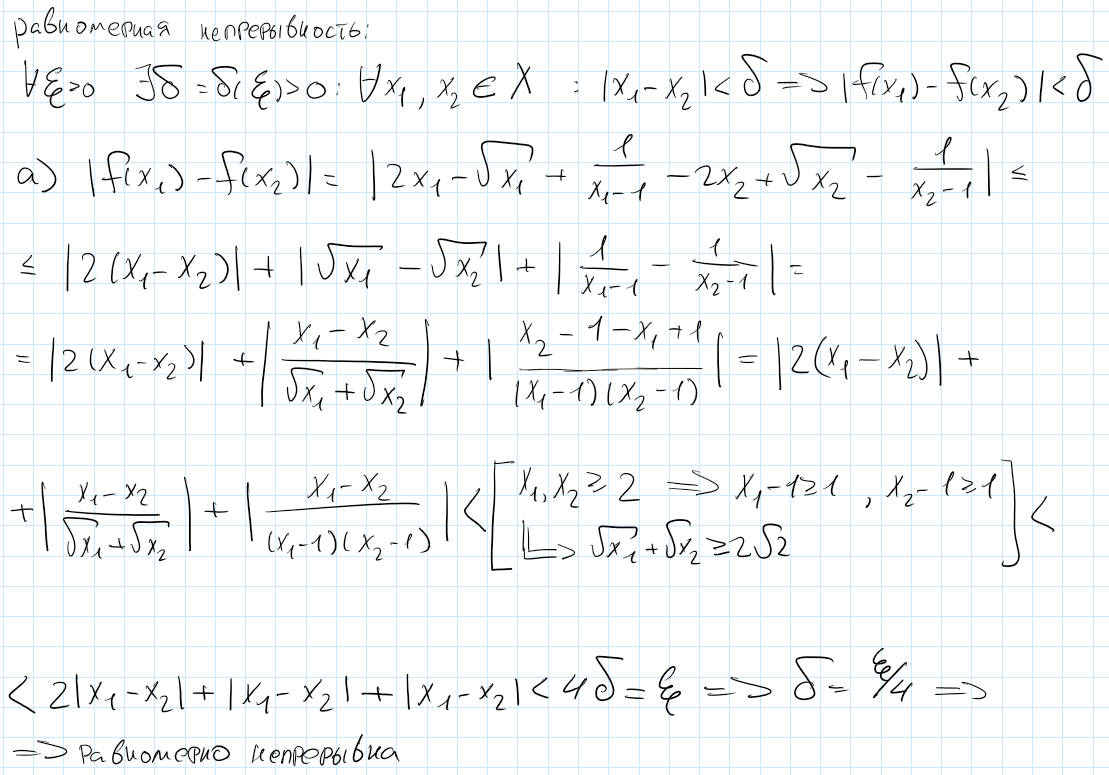
\includegraphics[width=\textwidth]{images/img11}
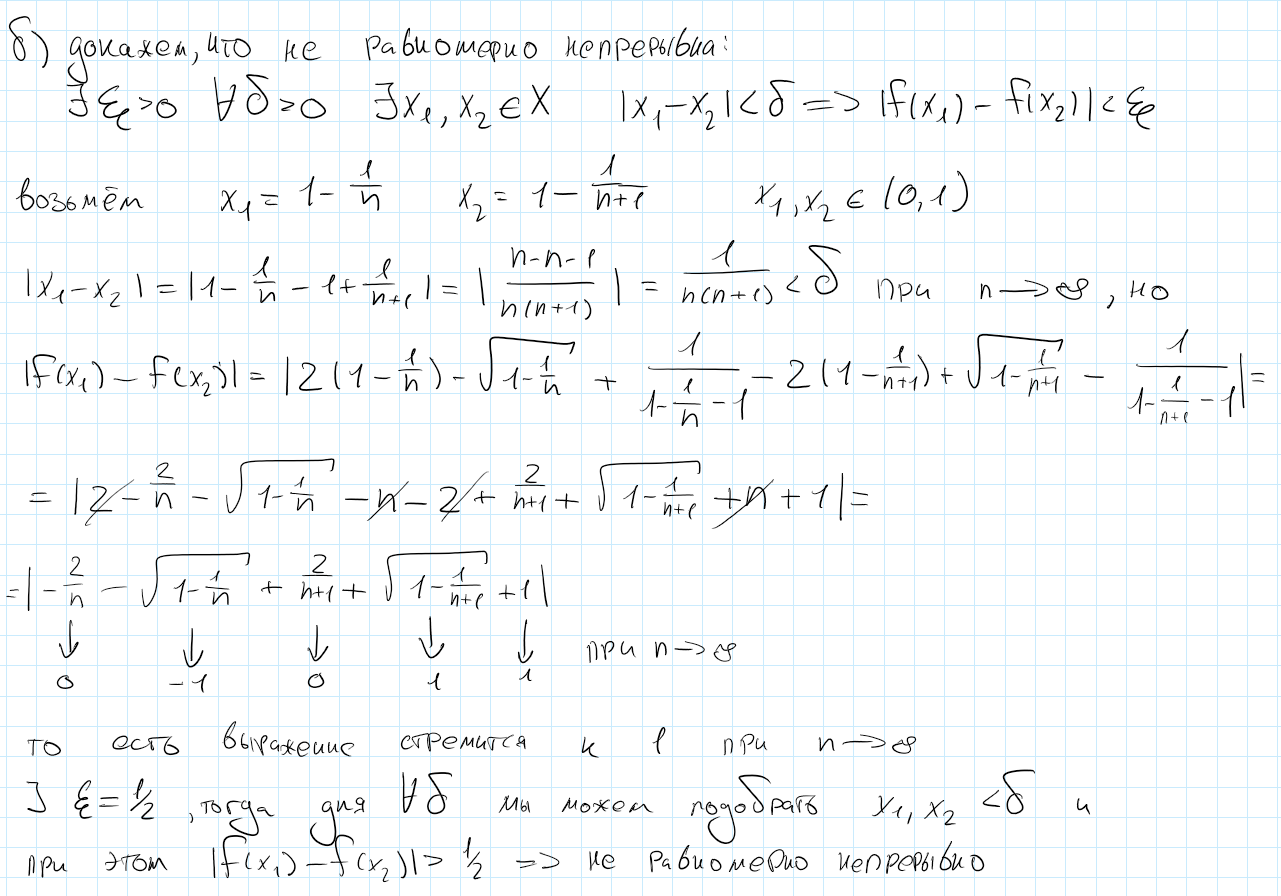
\includegraphics[width=\textwidth]{images/img12}
\newpage

\section*{Задание 2}
\textf{Преобразовать выражение к интегральной сумме, доказать существование соответствующего интеграла и найти предел.\\}
{\large
    \[
        \lim\limits_{n \to \infty} (\frac{n}{n^2 + 1} + \frac{n}{n^2 + 4} + \cdots + \frac{n}{n^2 + n^2})
    \]
}
\textbf{\Large Решение:\\}

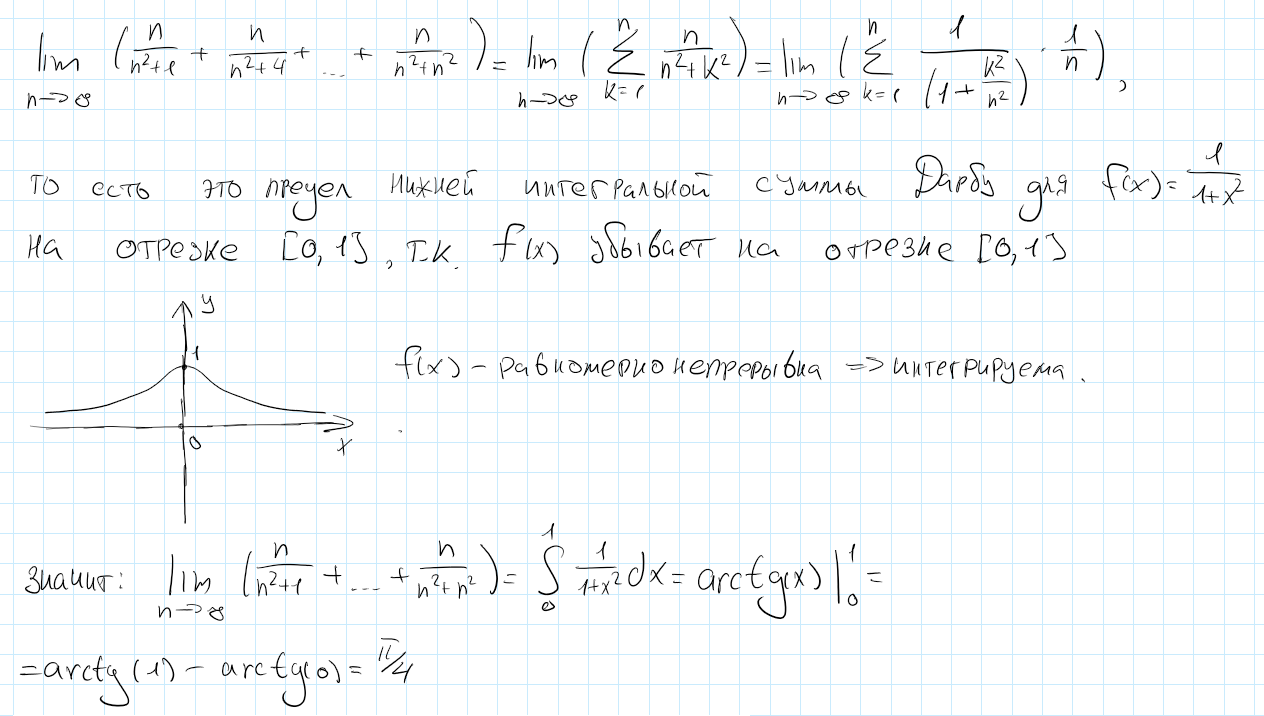
\includegraphics[width=\textwidth]{images/img21}
\newpage

\section*{Задание 3}
\textf{Найти площадь фигуры, ограниченной кривой, заданной параметрически. Сделать рисунок.}
{\large
    \[
        x = n\cos t - \cos(nt) \quad y = n\sin t - \sin(nt) \quad (n \in \mathbb{N})
    \]
}
\textbf{\Large Решение:\\}

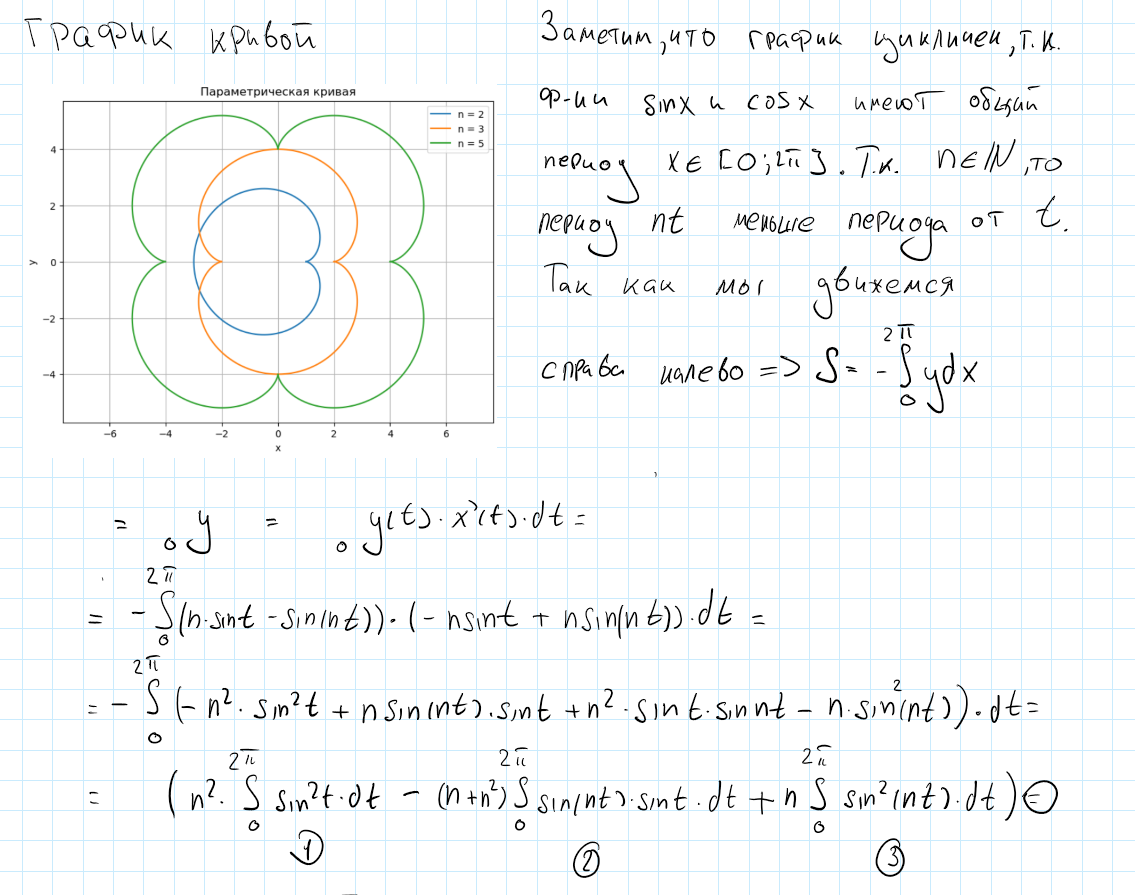
\includegraphics[width=\textwidth]{images/img31}
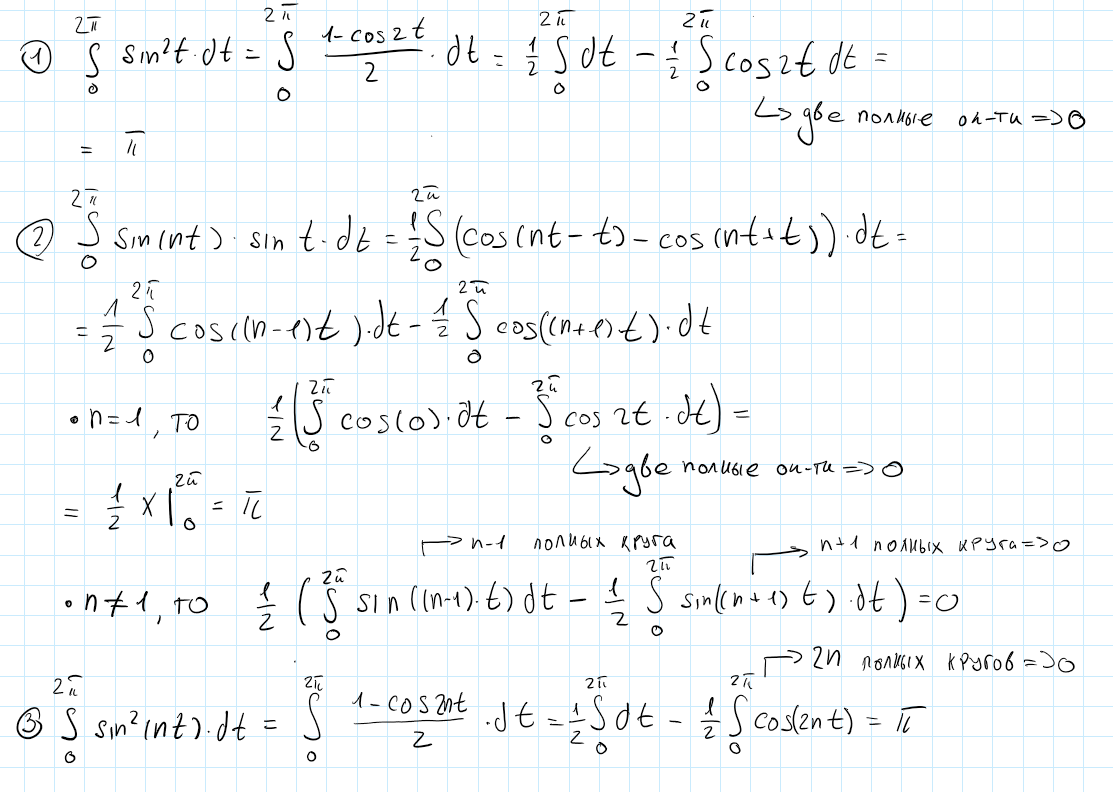
\includegraphics[width=\textwidth]{images/img32}
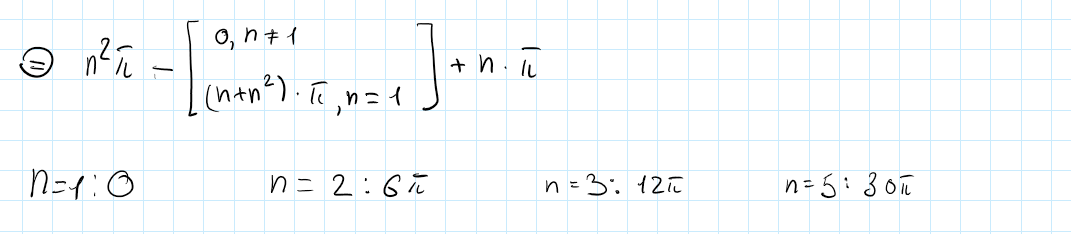
\includegraphics[width=\textwidth]{images/img33}
\newpage

\section*{Задание 4}
\textf{Кривая задана как пересечение поверхностей, заданных данными у равнениями в декартовых координатах. Задайте кривую параметрически и найдите длину кривой}
{\large
    \[
        x^6 + y^6 = a^2x^2y^2
    \]
}
\textbf{\Large Решение:\\}

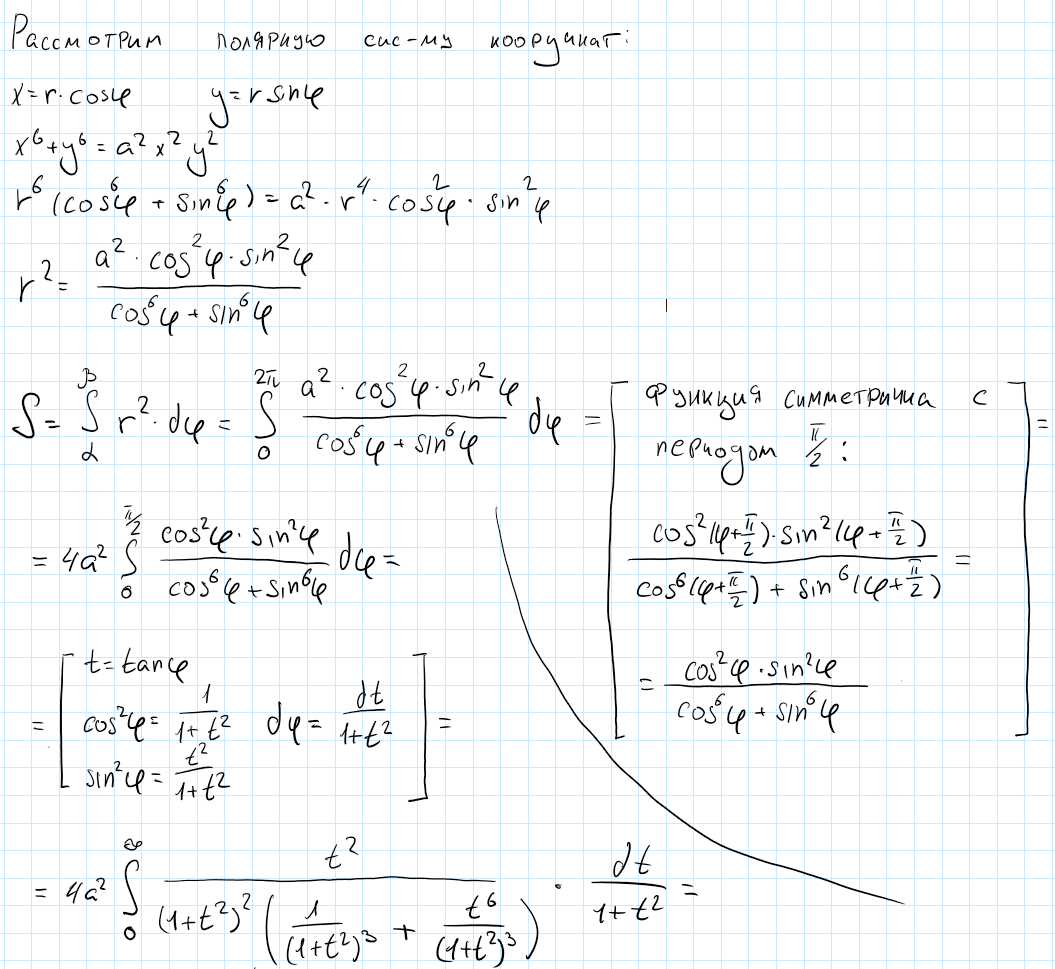
\includegraphics[width=\textwidth]{images/img41}
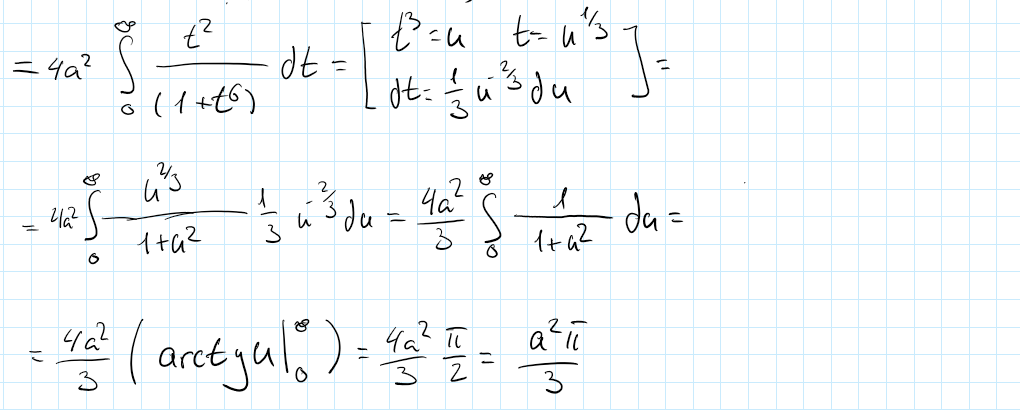
\includegraphics[width=\textwidth]{images/img42}
\newpage

\section*{Задание 5}
\textf{Найти длину кривой, заданной параметрически. Сделать рисунок.}
{\large
    \[
        x^2 + y^2 + z^2 = 9, |z| = y
    \]
}
\textbf{\Large Решение:\\}

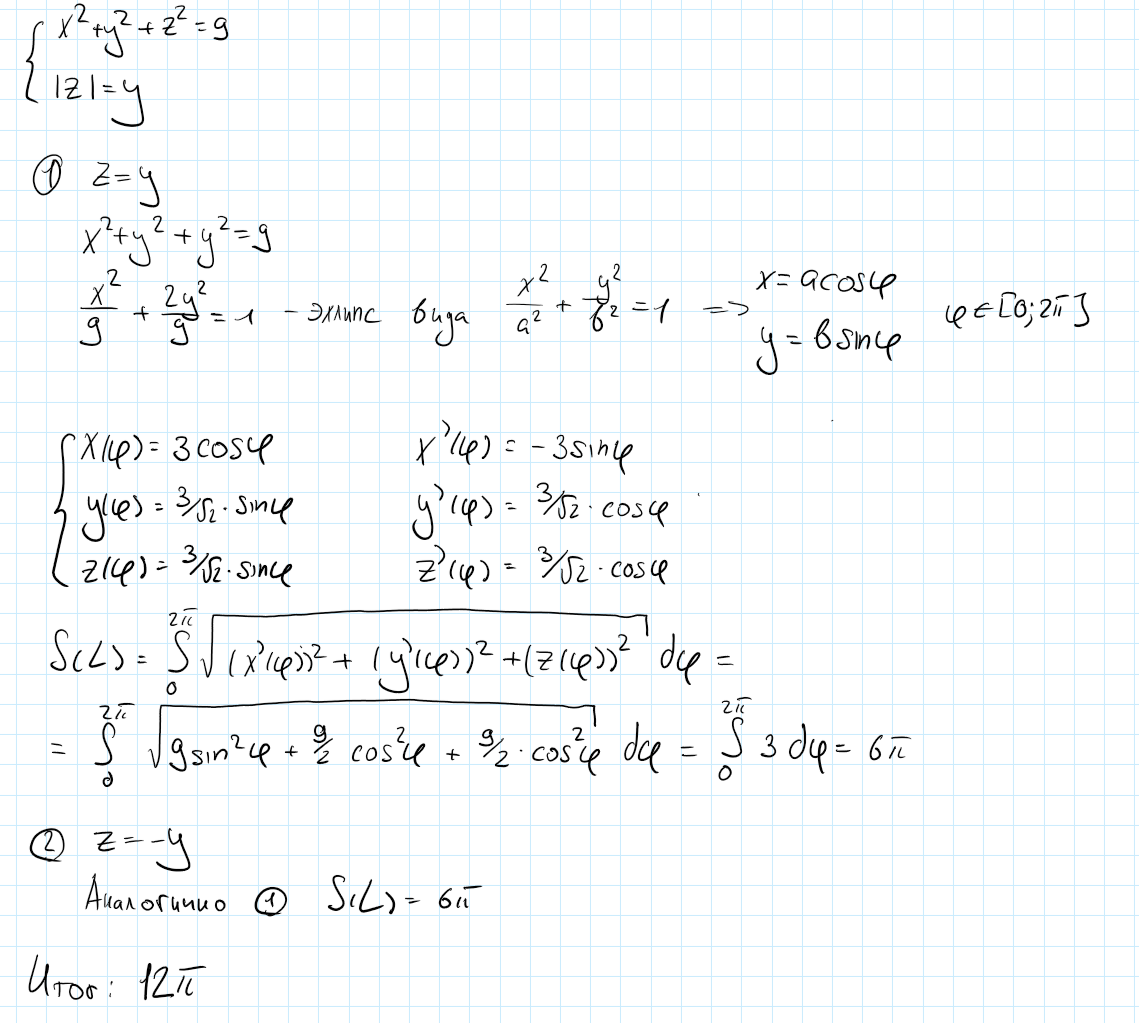
\includegraphics[width=\textwidth]{images/img51}
\newpage

\section*{Задание 6}
\textf{Исследовать интеграл на сходимость в каждой особой точке. Если функция меняет знак - на абсолютную и условную сходимость.}
{\large
    \[
        \int\limits_{1}^{\infty} \frac{\cos x}{x} \left( \frac{x + 1}{x} \right)^x \, dx
    \]
}
\textbf{\Large Решение:\\}

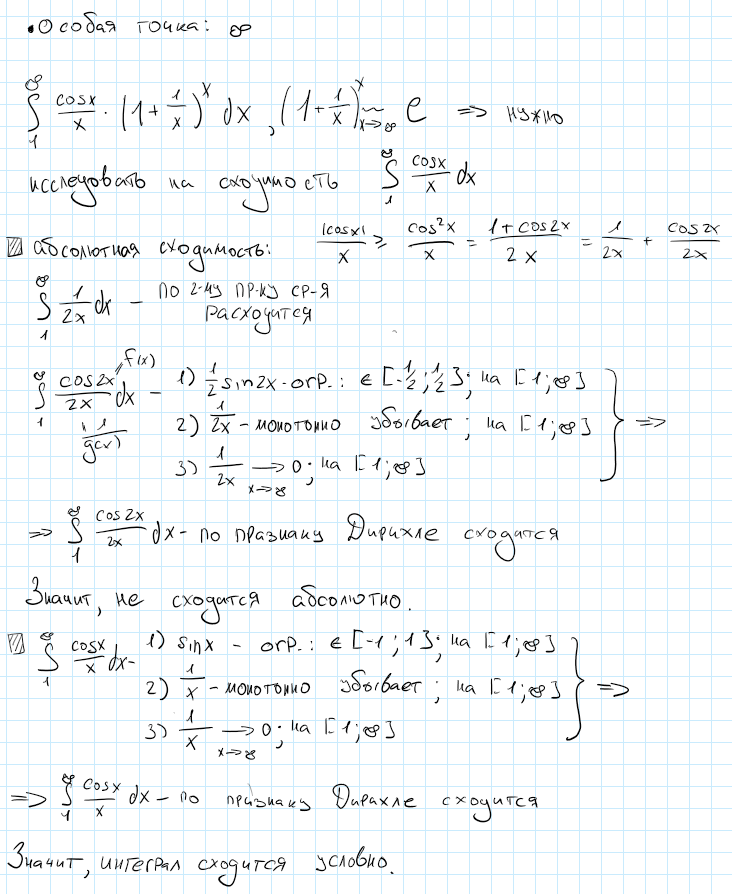
\includegraphics[width=\textwidth]{images/img61}
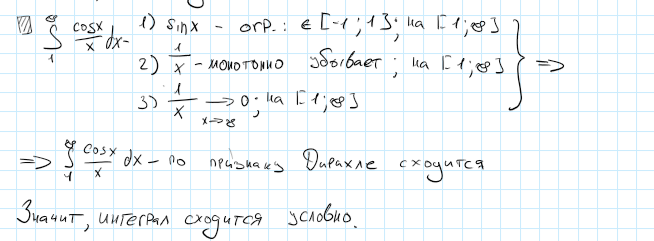
\includegraphics[width=\textwidth]{images/img62}
\newpage

\section*{Задание 7}
\textf{Исследовать интеграл на сходимость в каждой особой точке. Если функция меняет знак - на абсолютную и условную сходимость.}
{\large
    \[
        \int\limits_{0}^{\infty} \frac{\ln(1 + x + x^2) + \ln(1 - x + x^2)}{x^{3/2} (e^{x} + 1)} \, dx
    \]
}
\textbf{\Large Решение:\\}

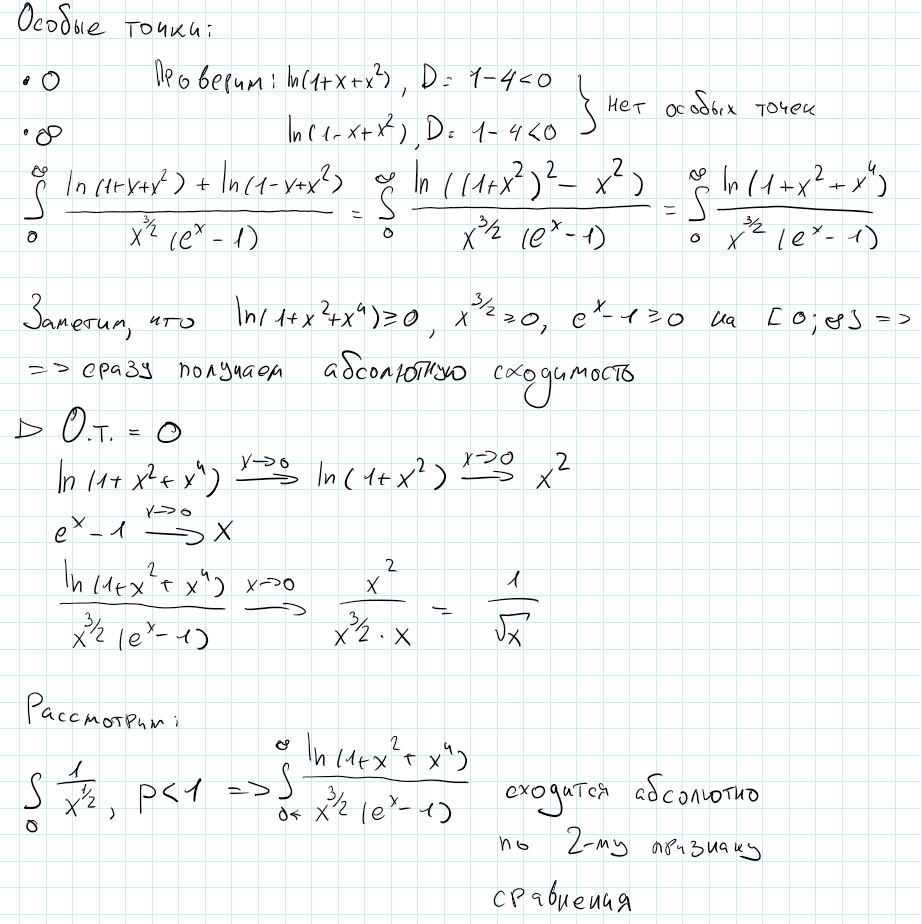
\includegraphics[width=\textwidth]{images/img71}
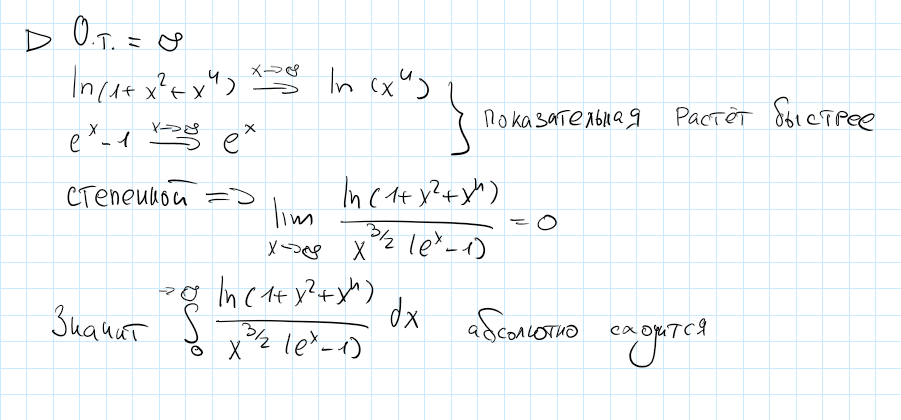
\includegraphics[width=\textwidth]{images/img72}
\newpage

\section*{Лабараторная работа 1. Аналитический этап.}
{\large
    \[
        f(x) = \sqrt {e^x} + 4x,\quad [a, b] = [0, 2]
    \]
}

\textf{1. Составить верхнюю и нижнюю суммы Дарбу, вычислить эти суммы. При необходимости, разбивать функцию на участки монотонности.\\\\}
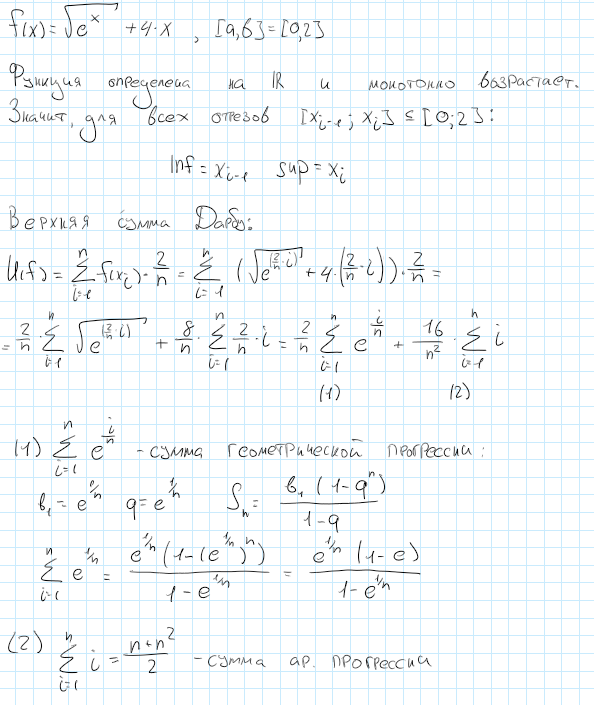
\includegraphics[width=\textwidth]{images/lab/img}
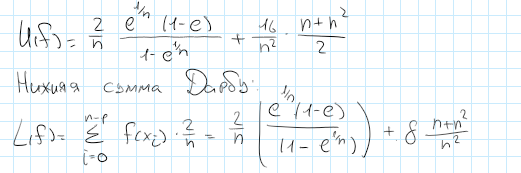
\includegraphics[width=\textwidth]{images/lab/img_1}
\newpage

\textf{2. Проверить критерий Римана интегрируемости функции.\\\\}
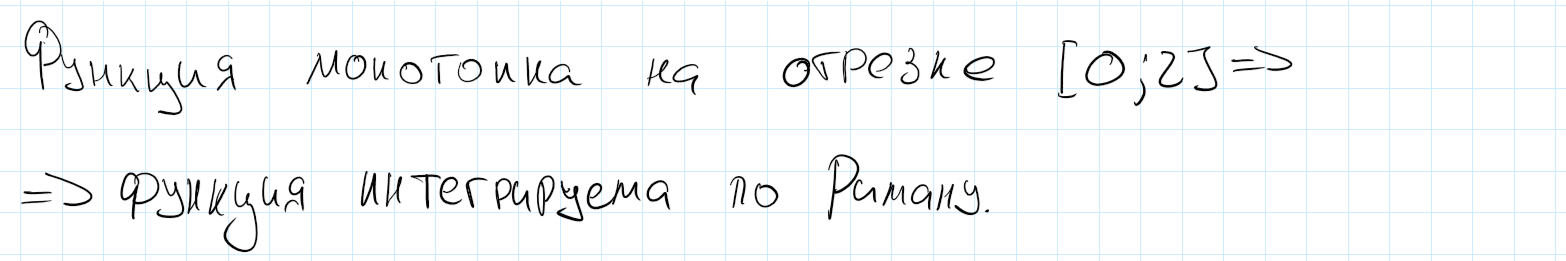
\includegraphics[width=\textwidth]{images/lab/img_2}
\newpage

\textf{3. Найти интегралы Дарбу и сделать вывод об интегрируемости функции, в том числе о значении интеграла\\\\}
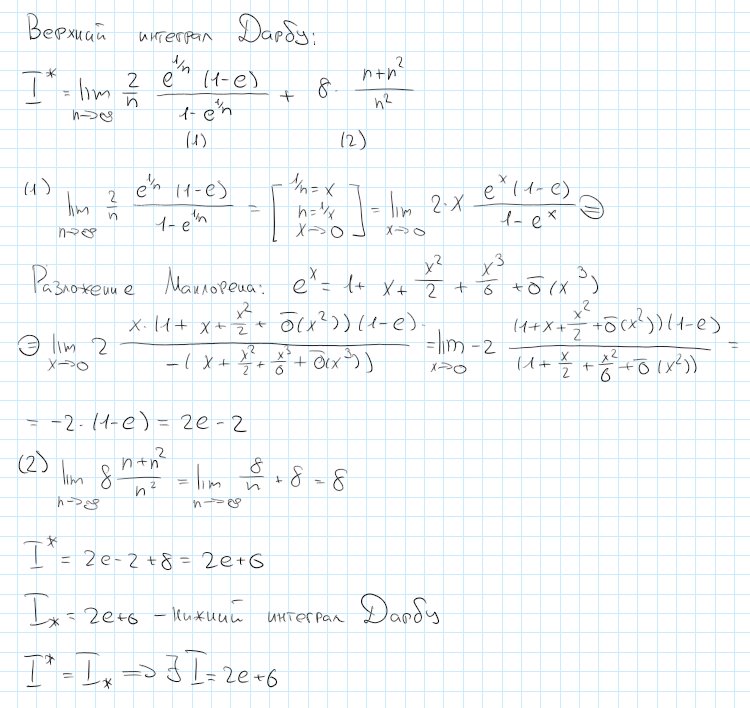
\includegraphics[width=\textwidth]{images/lab/img_3}
\newpage

\textf{4. Подобрать еще одно достаточное условие интегрируемости данной функции, отличное от упомянутых критериев и проверить его.\\\\}
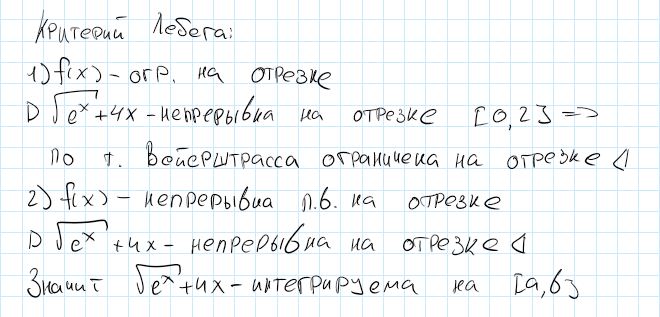
\includegraphics[width=\textwidth]{images/lab/img_4}
\newpage

